\documentclass{beamer}
\usepackage{pgfpages}
\usepackage[francais]{babel}
\usepackage[T1]{fontenc}
\usepackage[utf8]{inputenc}
\usepackage{amsmath,amsthm}
\usepackage{amsfonts,amssymb}

%%%%%%%%%%%%%%%%%%%%%%%%%%%%%%%%%%%%%%%%%%%%%%%%%%%%%%%%%%%%%%%%%%%%%%%%%%%%%%%
%THEMES DU DOCUMENT
%%%%%%%%%%%%%%%%%%%%%%%%%%%%%%%%%%%%%%%%%%%%%%%%%%%%%%%%%%%%%%%%%%%%%%%%%%%%%%%

%– th`emes globaux~: albatross, beetle, crane, fly, seagull.
%– th`emes internes~: lily  orchid, rose.
%– th`emes externes~: whale, seahorse, dolphin
%JuanLesPins Malmoe PaloAlto Berlin Boadilla Copenhagen Hannover Goettingen Montpellier Rochester
%Madrid Antibes Singapore Szeged Warsaw, thème par défaut Ilmenau Luebeck AnnArbor CambridgeUS Dresden

%themes de polices~: professionalfonts serif structurebold structureitalicserif structuresmallcapsserif


\usetheme{Warsaw}
%\usecolortheme{dolphin}
\usefonttheme{structurebold}
%\useinnertheme{nom du theme interne}
%\useoutertheme{split}

%%%%%%%%%%%%%%%%%%%%%%%%%%%%%%%%%%%%%%%%%%%%%%%%%%%%%%%%%%%%%%%%%%%%%%%%%%%%%%%%%%%%%%%%
%AUTRES COMMANDES PRÉLIMINAIRES
%%%%%%%%%%%%%%%%%%%%%%%%%%%%%%%%%%%%%%%%%%%%%%%%%%%%%%%%%%%%%%%%%%%%%%%%%%%%%%%%%%%%%%%%%

\AtBeginSection[]{% génère une tableofcontents au début de chaque section
  \begin{frame}
  \frametitle{Sommaire}
	\tableofcontents[sectionstyle = show/shaded,subsectionstyle = show/show/shaded]
  \end{frame}
}

\setbeamertemplate{itemize item}[triangle]
\setbeamertemplate{enumerate item}[square]
\setbeamertemplate{blocks} [rounded] [shadow=true]

\setbeameroption{show notes}%%ou hide notes
%%\setbeameroption{show notes on second screen=right}


\title{Réunion de lancement}
\subtitle{PSC INF02~: Synthétiseur automatique de documents}
\author{}
\institute{École polytechnique}
\date{}

\logo{
\includegraphics[height=0.8cm]{logohori.eps}}

%%%%%%%%%%%%%%%%%%%%%%%%%%%%%%%%%%%%%%%%%%%%%%%%%%%%%%%%%%%%%%%%%%%%%%%%%%%%%%%%%%%
%DEBUT DU DOCUMENT
%%%%%%%%%%%%%%%%%%%%%%%%%%%%%%%%%%%%%%%%%%%%%%%%%%%%%%%%%%%%%%%%%%%%%%%%%%%%%%%%%%%

\begin{document}




%%page de titre
\begin{frame}
  \titlepage{}
\end{frame}

%% sommaire %%
% \begin{frame}
% \frametitle{Sommaire}
% \tableofcontents
% \end{frame}


%%%%%%%%%%%%%%%%%%%%%%%%%%%%%%%%%%%%%%%%%%%%%%%%%%%%%%%%%%%%%%%%%%%%%%%%%%%%
%VRAI DEBUT DU DOCUMENT
%%%%%%%%%%%%%%%%%%%%%%%%%%%%%%%%%%%%%%%%%%%%%%%%%%%%%%%%%%%%%%%%%%%%%%%%%%%%

\section{Introduction}

    \begin{frame}%[allowframebreaks=0.8]
    \frametitle{Cadre du problème}%cadre général
        %%à l'ère du big data, une grande partie de ces données sont textuelles

        \begin{block}{Nécessité et difficulté de résumés automatiques}
            \begin{itemize}
                \item De grandes quantités de données textuelles
                \item Une grammaire complexe (langage naturel)
                \item Beaucoup de prérequis de bon sens ou de culture générale %exemple ?
            \end{itemize}
        \end{block}


        \begin{block}{Plusieurs solutions envisageables}
            \begin{itemize}
                \item «~Comprendre~» l'information du texte et la retranscrire~: \textbf{résumé abstractif}
                \item Analyser le texte de façon statistique et en extraire des phrases~: \textbf{résumé extractif} %dans la littérature
            \end{itemize}
        \end{block}
    \end{frame}


    \begin{frame}
    \frametitle{Notre projet~: Synthétiseur automatique de documents}
        Nous voulons résumer un texte en langage naturel, de façon abstractive.

        Le résumé final ne sera pas une simple copie des phrases importantes du texte.
    \end{frame}


\section{Structure du projet}

    \subsection{Le projet}

        \begin{frame}
        \frametitle{Le synthétiseur en six étapes}

            \begin{columns}[t]
                \begin{column}{6cm}
                    \begin{enumerate} %éviter la liste
                        \item Analyse syntaxique
                        % ie la grammaire. Nos exigences devraient entrer dans le champ des possibilités des outils libres déjà existants
                        \item Repérage des entités.
                        %les entités ne sont rien d'autre que des concepts importants
                        \item Connaissances des liens entre entités.
                        %liens qui sont donnés par FB~: Zlatan est un joueur de foot par exemple
                        \item Analyse des concepts.
                        %il s'agit de relier tous les mots à des concepts
                        \item Approfondissement des liens entre les concepts.
                        %explicité dans la suite
                        \item Génération de texte simple
                    \end{enumerate}
                \end{column}
                %à droite, ce que ça donne aux différents stades

                \begin{column}{6cm}
                    \begin{itemize}
                        \item Sujet, Verbe, Objet\ldots{}
                        \item Zinedine Zidane\ldots{}
                        \item Zidane est un joueur de football\ldots{}
                        \item Le football est un sport\ldots{}
                        \item Zinedine Zidane est donc un sportif.
                        \item Sujets-Actions-Objets-Compléments
                    \end{itemize}
                \end{column}
            \end{columns}
        \end{frame}

        \begin{frame}
        \frametitle{Déroulement du projet}
            \begin{enumerate}
                \item Étude statistique
                \item Étude syntaxique et linguistique
                \item Étude «~intelligente~» %but/gros du PSC
                \item Génération et étude de la qualité du résumé
            \end{enumerate}
        \end{frame}

    \subsection{Organisation du travail}

        \begin{frame}
        \frametitle{Méthodes de travail}
        	\begin{itemize}
        		\item Des réunions hebdomadaires, pour~:
        		\begin{itemize}
        			\item Faire le point sur le travail effectué dans la semaine;
        			\item Rendre compte et résoudre les difficultés rencontrées;
        			\item Définir les axes prioritaires pour la semaine à venir.
        		\end{itemize}
        		\item Un répertoire partagé (git) pour une gestion pratique des fichiers.
        	\end{itemize}
        \end{frame}

        \begin{frame}
        \frametitle{Moyens utilisés}
            De nombreux outils \textit{open-source} ou libres, notamment~:
            \begin{itemize}
                \item Freebase
                \item WordNet (Princeton)
                \item nltk (librairie python)
            \end{itemize}
        \end{frame}


\section{Étude statistique}
    \begin{frame}
    \frametitle{TF-IDF(Term Frequency-Inverse Document Frequency)}
        \begin{itemize}
            \item TF: la fréquence d'un terme est le nombre d'occurrences de ce terme dans le document considéré.
            \item IDF: la fréquence inverse de document est une mesure de l'importance du terme dans l'ensemble du corpus.
                $IDF_{i}=log \frac{|D|}{|d_{j}\,:\,t_{i}\in d_{j}|}$
            \item TF-IDF: le multiple de TF et IDF.\newline{}
                \textbf{Exemple: le poids du mot i sur le document j}
                $TFIDF_{i,j} = TF_{i,j} \times IDF_{i}$
        \end{itemize}
    \end{frame}

    \begin{frame}
    \frametitle{Utilisations du TF-IDF}
        \begin{itemize}
        \item Similarité de documents:\newline{}
        On mesure la coprésence de mots-clés entre deux documents.
        \item Résumé extractif:
            \begin{itemize}
                \item On trie les mots selon leur valeurde TF-IDF;
                \item On calcule les valeurs des phrases à partir des mots-clés;
                \item On extrait les phrases les plus importantes.
            \end{itemize}
        \end{itemize}
    \end{frame}

\section{Structure de l'analyseur}%Guillaume
    \begin{frame}
        \frametitle{Exemple - Fil rouge}
        Phrase à analyser:\newline{}
        "Wayne Rooney celebrated his appointment as England captain with the winner against Norway on a night when
        fans turned their back on the team following their dismal World Cup exit."
    \end{frame}

    \subsection{Réseau de concepts}
        \begin{frame}
        \frametitle{Réseau de concepts}
            \begin{itemize}
                \item Graphe de concepts (objets, actions ou idées plus abstraites) reliés entre eux;
                \item Deux concepts sont proches s'il est pertinent de penser au second après avoir rencontré le premier;
                \item Modélise une certaine compréhension du monde;
                \item Capable d'apprendre et d'évoluer à partir des résultats d'une analyse de texte.
            \end{itemize}
        \end{frame}

        \begin{frame}
        \frametitle{Exemple}
            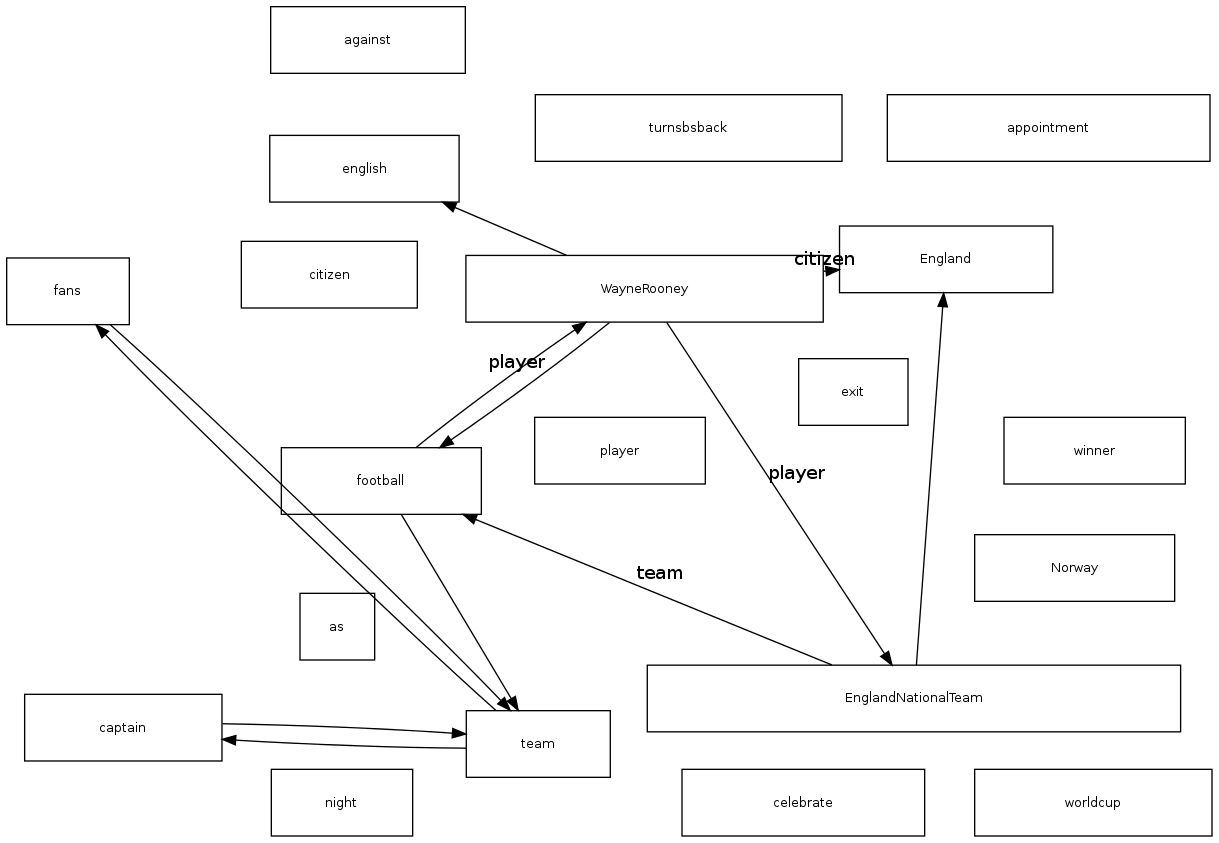
\includegraphics[height=0.8\textheight]{RC/figures/RCetape0.png}
        \end{frame}

        \begin{frame}
        \frametitle{Concept clé: l'activation}
            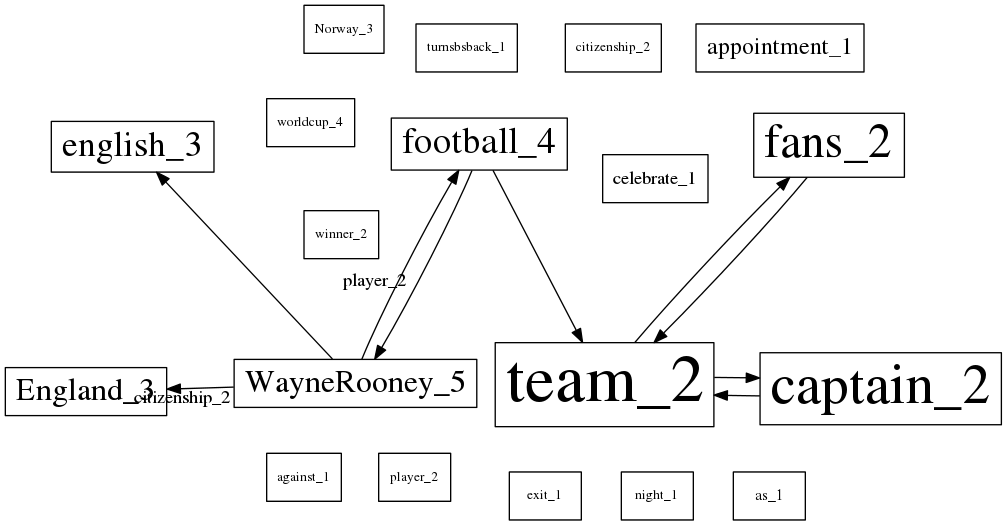
\includegraphics[height=0.8\textheight]{RC/figures/RCetape30.png}
        \end{frame}

    \subsection{Workspace}
        \begin{frame}
        \frametitle{Workspace}
            \begin{itemize}
                \item Zone de travail qui contient les \textit{instances} des concepts rencontrés et des structures en cours de construction;
                \item Modélise la progression de la compréhension du texte;
                \item Quand l'analyse est terminée, les structures présentes dans le Workspace représentent la compréhension du texte qu'a acquise l'analyseur.
            \end{itemize}
        \end{frame}

        \begin{frame}
        \frametitle{Exemple}
        \end{frame}

    \subsection{Workers}
        \begin{frame}
        \frametitle{Workers}
            Ensemble de méthodes permettant d'extraire de l'information du texte et du réseau de concepts.\newline{}
            Par exemple:
            \begin{itemize}
                \item Lecture mot-à-mot du texte;
                \item Identification les références à un même objet;
                \item Importance des mots selon l'ordre du texte, les paragraphes, le titre.
            \end{itemize}
        \end{frame}

    \subsection{Synthèse}
        \begin{frame}
        \frametitle{Synthèse}
            Fonctionnement de l'analyseur:
            \begin{itemize}
                % \item Le réseau de concepts contient des connaissances \textit{a priori};
                \item La lecture du texte active le réseau de concepts;
                \item Les concepts activés sont instanciés dans le workspace;
                \item Les workers travaillent dans le workspace et créent des structures;
                \item À la fin, les structures les plus importantes permettent d'obtenir une synthèse du texte.
            \end{itemize}
        \end{frame}

\begin{frame}
	\frametitle{Dans l'immédiat...}
	\begin{itemize}
		\item Finir l'implémentation de TF-IDF ;
		\item Utiliser NLTK pour l'analyse syntaxique ;
		\item Étoffer le réseau de concepts.
	\end{itemize}
\end{frame}

\end{document}
